\section{Results} \label{results}
After removing spoofed data and other devices with a single record we detected 16571 unique devices during the festival period of Haven and 28328 devices during the festival period of Northside. Of these 109 (0.7\%) were deemed stationary and 8804 (53.1\%) noise in the Haven data, while 167 (0.6\%) were deemed stationary and 8041 (28.4\%) noise in the Northside data (see Section~\ref{sec:filtering}).

The data of the remaining 7738 devices recorded for the Haven festival and 20239 devices recorded at Northside was used in the following analysis.  

\subsection{Timelines}
For a basic analysis we decided to show the number of unique devices seen at chosen stage over time for each of the festivals. Figure~\ref{fig:stage_timelines} shows that the amount of devices, i.e. visitors, correlates with the time periods during which there was a concert at the corresponding stage. In addition, we see an expected increase of visitors before the start of each festival day towards the first concert and an expected decrease after the last concert of each day.

\begin{figure}[tb]
  \centering
  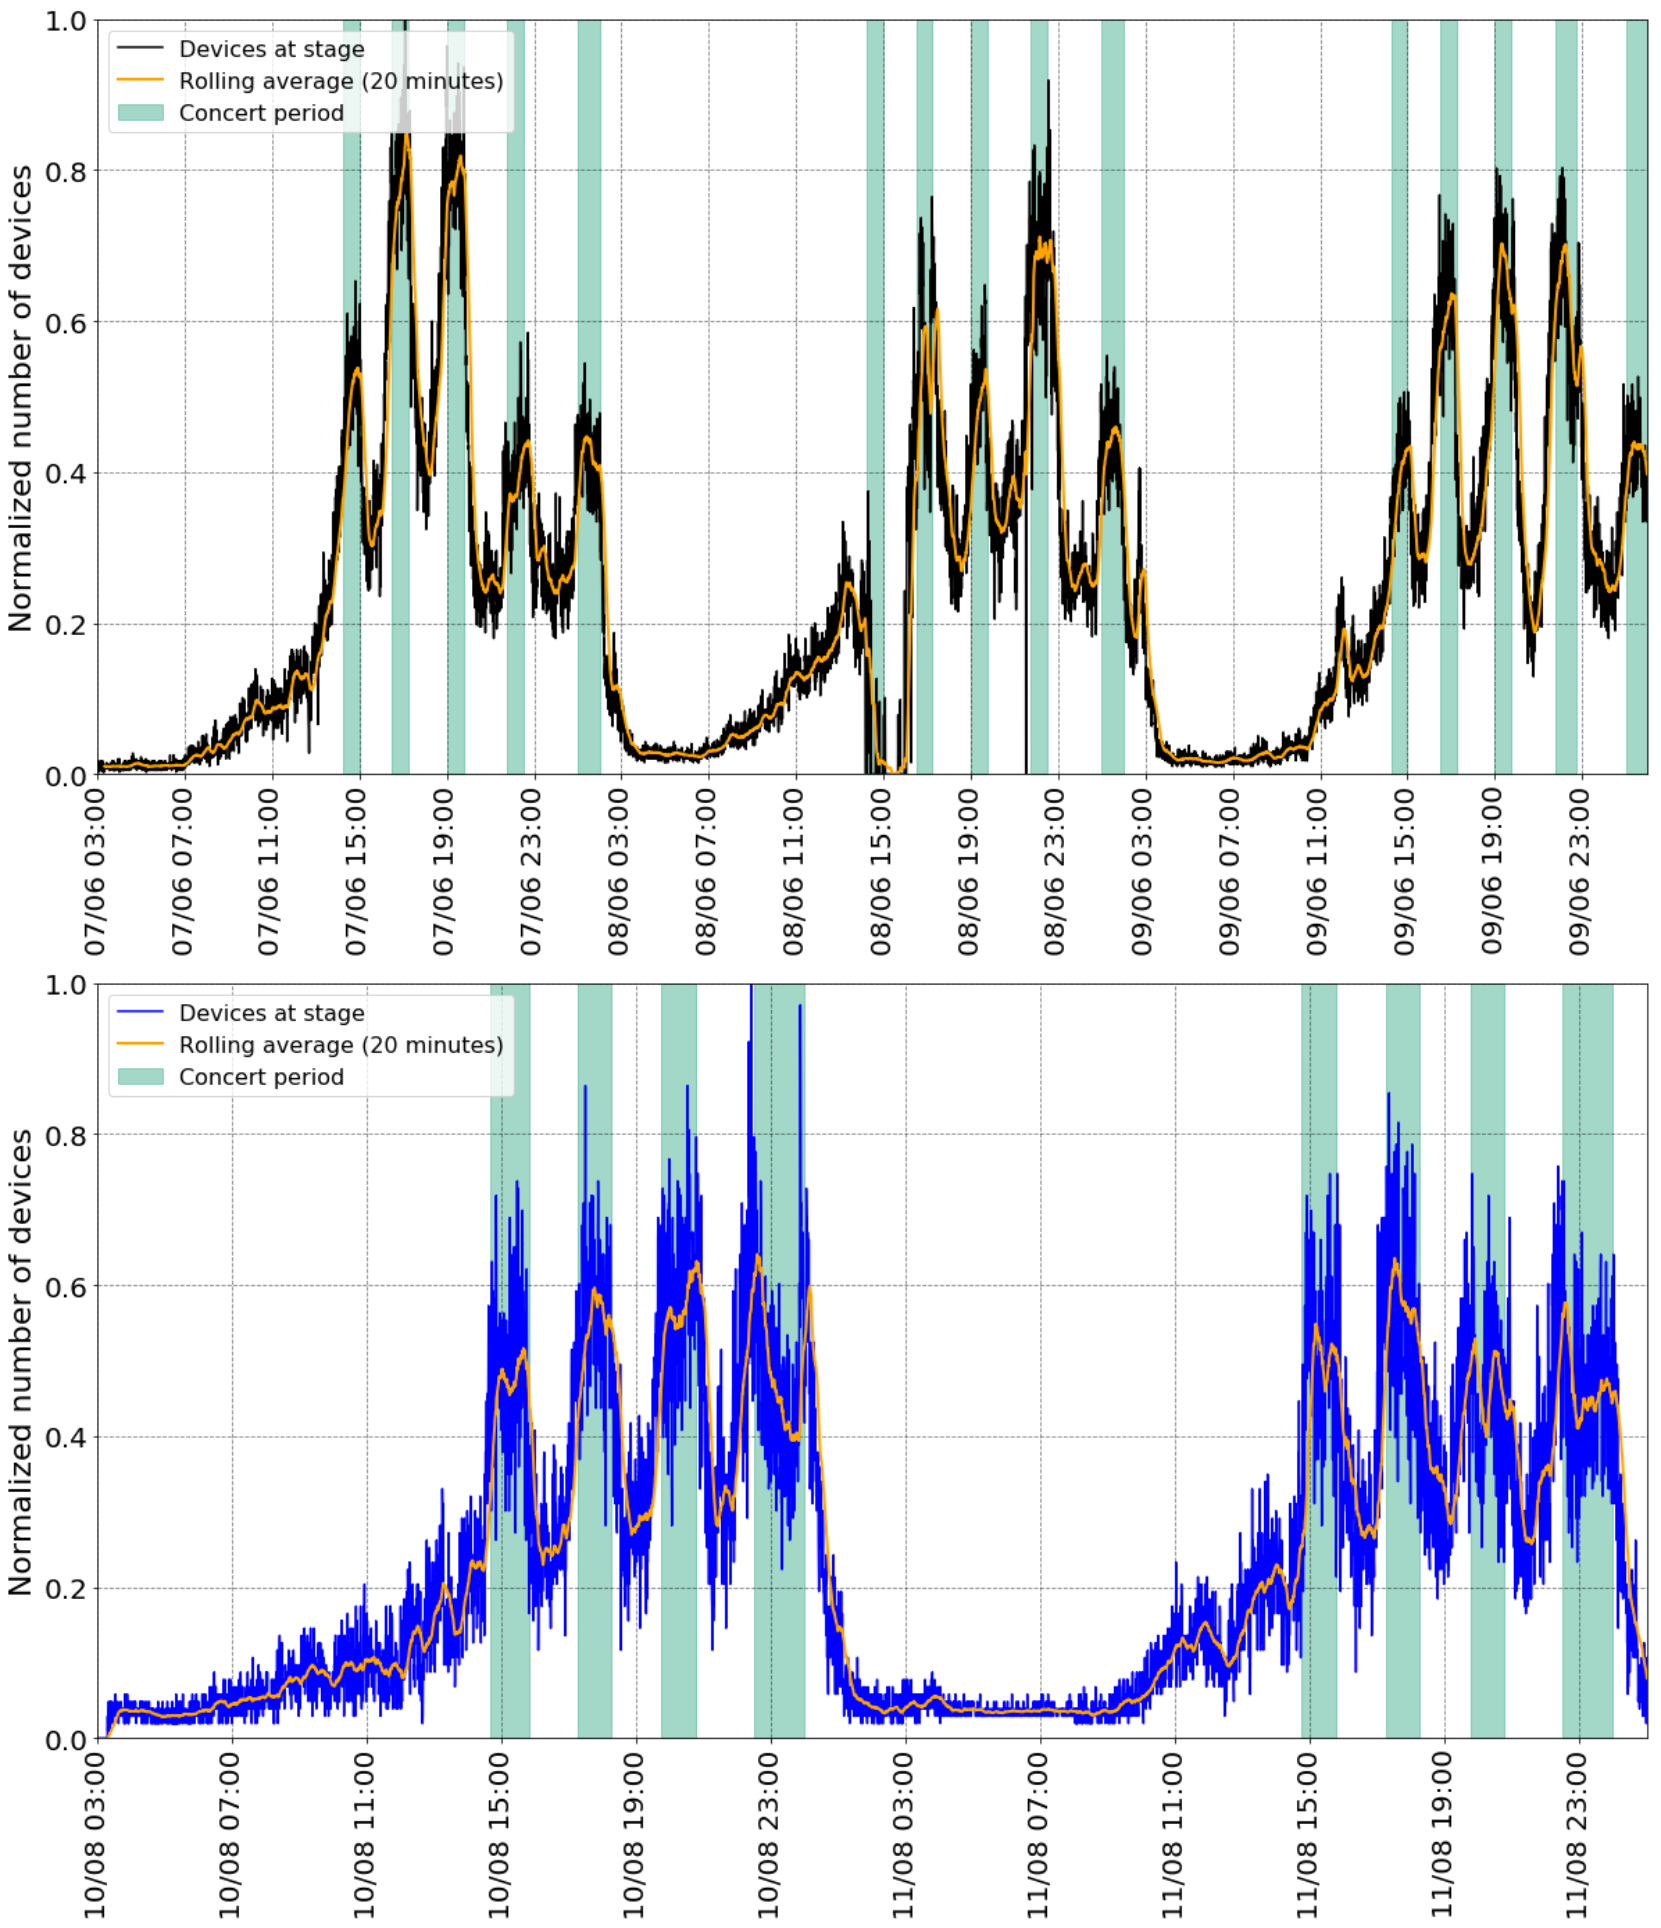
\includegraphics[width=\linewidth]{figs/stage_timelines.png}
  \caption{Amount of devices (Nortside: black, Haven: blue) at a chosen stage throughout the festival period normalized to be between 0 and 1. The orange line shows the average of devices over the past 20 minutes. The shaded areas denote the periods during which there was a concert at the corresponding stage. Top: Northside. Bottom: Haven.}
  \label{fig:stage_timelines}
\end{figure}

\subsection{Feature analysis}
Figure~\ref{fig:features} A--C show the distribution of three computed features (see Section~\ref{sec:dataproc}) in form of a boxplot over all visitors for both festivals separately. While 75\% of the visitors at Northside stayed at least 3.6 hours, at Haven only 60\% stayed that long. Similarly, only 25\% of Haven's visitors stayed more than 7.2 hours, while almost half (46\%) of Northside's visitors stayed longer than that. This can be explained by the different size of the festivals, Haven's close location to Copenhagen's city center and exceptionally bad weather during Haven causing visitors to leave the festival.

Beside differences in visiting time, it is also possible to see differences of the sensor set-up. Visitors at Northside where seen at more sensors (13 on average) an switched more often between them (40 times on average) than at Haven (seen at 8 sensors and switched 29 times on average). This means we had a better coverage and granularity at Northside festival than at Haven.

\begin{figure}[tb]
  \centering
  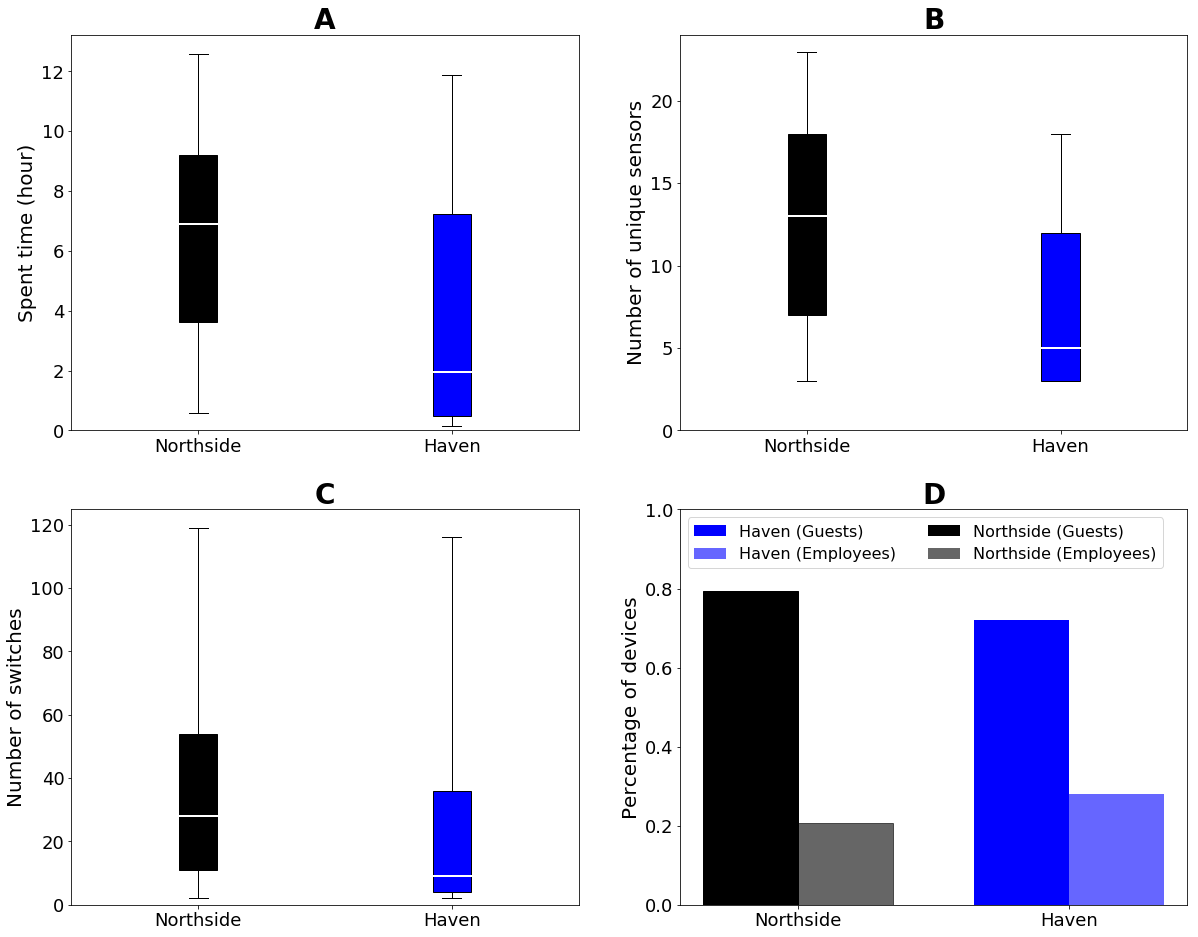
\includegraphics[width=\linewidth]{figs/features_boxplot.png}
  \caption{\textbf{A--C}: Boxplots showing the distribution for the three device features (\textbf{A} spent time, \textbf{B} number of sensors, \textbf{C} number of switches) over all visitor at Northside (black) and Haven (blue). Marked are the 5\% (lower whisker), 50\% (white line) and 95\% (upper whisker) percentile. \textbf{D}: Amount of guests (solid bar) and employees or volunteers (transparent bar) in percentage for both Northside (black) and Haven (blue).}
  \label{fig:features}
\end{figure}